\chapter{Stand van zaken}
\label{ch:stand-van-zaken}
% Tip: Begin elk hoofdstuk met een paragraaf inleiding die beschrijft hoe
% dit hoofdstuk past binnen het geheel van de bachelorproef. Geef in het
% bijzonder aan wat de link is met het vorige en volgende hoofdstuk.

% Pas na deze inleidende paragraaf komt de eerste sectiehoofding.
Niet alles wat in dit onderzoek al is aangekaart, is gemakkelijk te begrijpen. Want natuurlijk zijn de begrippen zoals \emph{Kafka} en \emph{RabbitMq} niet voor iedereen even duidelijk. Ook de term microservices zal bij sommigen de wenkbrauwen wel eens doen fronsen. In dit hoofdstuk is het de bedoeling uit te leggen wat al deze begrippen betekenen. Na dit hoofdstuk zul je in staat zijn om met deze informatie te begrijpen wat er allemaal gebeurt in dit onderzoek.
\section{Microservices}

Microservices is een software architectuur. De applicatie bestaat uit meerdere kleinere componenten die samen één groot geheel vormen. Deze kleinere componenten zijn onafhankelijk van elkaar en hebben elk hun eigen proces. Deze software architectuur is vrij recent en is de laatste jaren een echte hype aan het worden.

Een belangrijke vraag is: waarom zijn microservices ontstaan? Server-side applicaties gebruiken meestel object-georiënteerde programmeertalen. Deze programmeer talen hebben abstracties om de complexiteit van hun programma's te behandelen in modules. Dit wordt ook wel eens `the monolith` genoemd. Dit is één groot geheel dat meestal uit drie lagen bestaat. De presentatielaag, de businesslaag en de datalaag. Deze lagen kunnen niet apart van elkaar gebruikt worden omdat ze verschillende resources met elkaar delen. Dit zorgt ervoor dat bij iedere wijziging in de applicatie, alle lagen opnieuw gereleased worden in een nieuwere versie. Je kan natuurlijk al raden dat dit in een grote applicatie niet de beste oplossing is. 

\begin{figure}[h!]
    \centering
    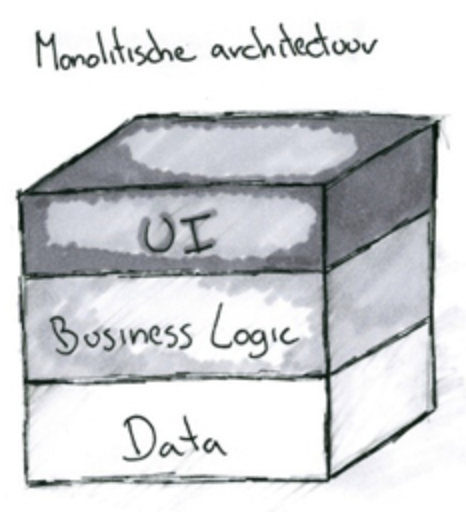
\includegraphics[width=80mm]{../monolith.png}
    \caption{Monolitische architectuur}
        
\end{figure}

Daarom is er een andere architectuur die een heel andere aanpak heeft, namelijk microservices. Dit bestaat uit verschillende kleinere componenten die indien nodig onafhankelijk van elkaar uitgevoerd kunnen worden. Bij deze aanpak is het ook belangrijk dat je uw services klein houdt. Hierdoor kunnen je services gemakkelijk hergebruikt, begrepen en opnieuw gebuild worden. Iedere microservice heeft dus maar 1 verantwoordelijkheid.

Omdat microservices op verschillende machines moeten kunnen draaien, bijvoorbeeld op verschillende besturingssystemen, is het beter om ze in te pakken samen met hun dependencies in een container. \emph{Docker} is een voorbeeld van een technologie die deze containers aanbiedt. Door microservices in containers te plaatsen, zorg je ervoor dat de uitvoering van deze services onafhankelijk gebeurt met andere applicaties op dezelfde machine. Containers zijn dus onafhankelijk van een besturingssysteem, hierdoor kunnen microservices op verschillende locaties gedraaid worden. Een van de voordelen hiervan is dat ze door containers in de cloud kunnen geprogrammeerd worden.

De vier grootste voordelen van microservices zijn: 
\begin{itemize}
    \item Schaalbaarheid
    \item Beperken complexiteit
    \item Verkorten time-to-market
    \item Autonomie van ontwikkelteams.
\end{itemize}

\emph{Kafka}, \emph{RabbitMq} en \emph{Google Pub/Sub} zijn technologieën die gebruikt kunnen worden om microservices te verwerken. Hieronder verklaren we hoe deze verschillende technologieën werken en waar de verschillen zich uiten.

 \autocite{Claudio2017} en \autocite{Velthoven2016}

\section{Kafka}

Wanneer je als bedrijf veel berichten binnen krijgt op een korte tijdsspanne, dan heb je natuurlijk een goed functionerende technologie nodig die al deze berichten kan verwerken. \emph{Kafka} is een voorbeeld van zo een technologie. Het is dus een berichtensysteem waarbij schaalbaarheid en redundantie een grote troef zijn. Bepaalde kernwoorden zijn belangrijk om de architectuur van \emph{Kafka} te begrijpen. Deze kernwoorden zijn: topics, producers, consumers en brokers.  

Topics zijn, zoals de naam al doet vermoeden, verschillende onderwerpen. Alle berichten zijn gegroepeerd in een van deze topics. Het formaat van een bericht kan verschillend zijn. Het type kan een gewone tekst zijn, kan van een Json-formaat zijn, of kan iets helemaal anders zijn. Het is mogelijk om zowel naar een specifieke topic een bericht te verzenden als te ontvangen. Dit brengt ons naadloos bij de volgende twee begrippen: producers en consumers. Als een producer kun je een bericht verzenden naar uw gewenste topic. Een consumer kan dan zelf bepalen van welke topic hij berichten wilt ontvangen. Het laatste woord dat nog moet verduidelijkt worden is een broker. \emph{Kafka} draait op een cluster. Iedere cluster bestaat uit één of meerdere nodes(servers). Zo een server noemen we een Kafka broker. Per Kafka cluster kunnen er verschillende producers en consumers zijn, zoals te zien is op figuur 2.2. 

\begin{figure}[h!]
    \centering
    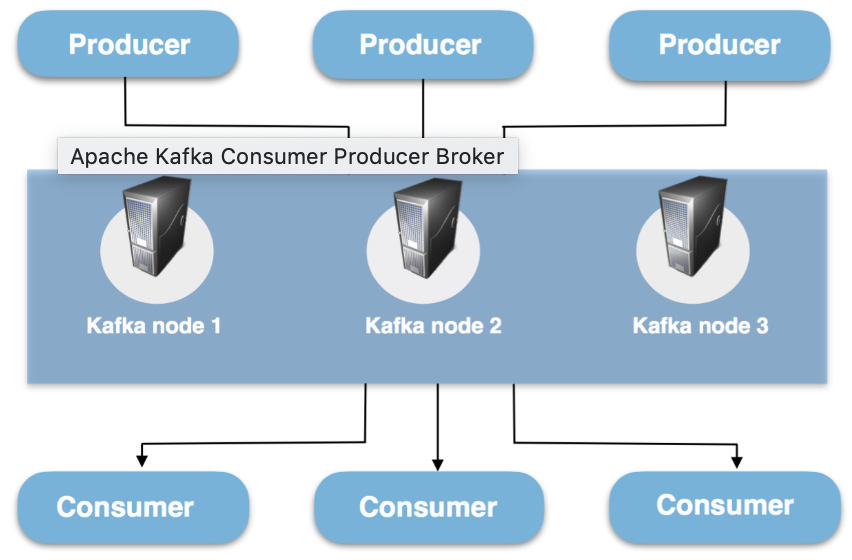
\includegraphics[width=80mm]{../kafkaCluster.png}
    \caption{Voorbeeld van een Kafka cluster, \autocite{Johansson2016}}
    
\end{figure}

 Een topic kan je verdelen in verschillende partities. Dit wil zeggen dat je uw data kunt verdelen in ongeveer gelijke groepen (brokers). Iedere partitie kan dan staan voor een specifieke groep data binnen een topic zodat je niet alle berichten altijd moet overlopen. Dit principe van verschillende partities wordt ook gebruikt bij traditionele databanken. Ook consumers kun je verdelen in verschillende partities, die samen één consumer-groep vormen. Door topics en consumers op deze manier op te delen, zorg je ervoor dat het mogelijk is dat meerdere consumers kunnen lezen van meerdere partities in een topic. Dit heeft als positief gevolg dat je meer berichten kunt verwerken binnen een bepaalde tijd. 
 
 Ieder bericht binnen een partitie heeft een offset. Dit is een identifier, waardoor het mogelijk is om de berichten te ordenen. Normaal gezien als je als consumer een subscriptie maakt op een topic, dan krijg je vanaf dit moment alle nieuwe berichten die binnen komen op de partitie waarop je een subscriptie hebt. Door een offset is het mogelijk om iets oudere berichten die op een partitie staan dan het moment dat je een subscriptie aangemaakt hebt, ook op te vragen. Op figuur 2.3 zie je een simpele voorstelling van een producer die berichten op een partitie van een topic plaatst. De cijfertjes stellen de offset voor van een bericht.
 \begin{figure}[h!]
     \centering
     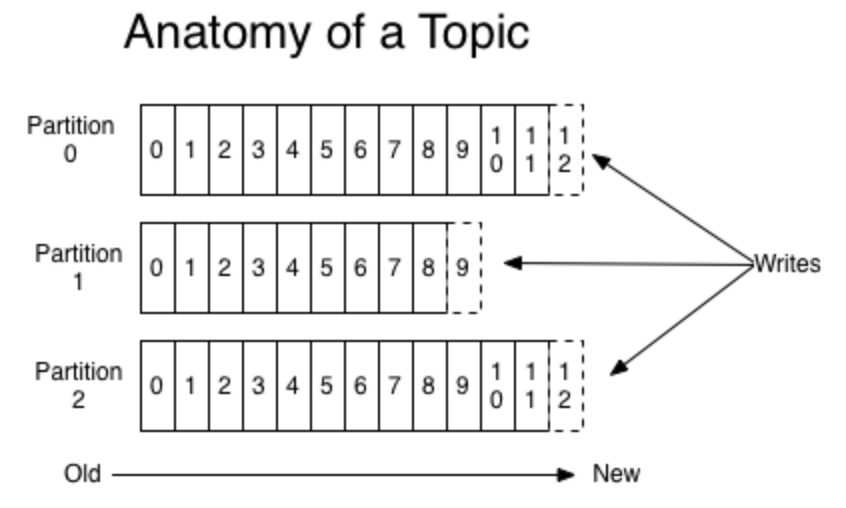
\includegraphics[width=80mm]{../kafkaOffset.png}
     \caption{Simpele voorstelling van de werking van een offset, \autocite{Sookocheff2015}}
     
 \end{figure}

Het is al even vermeld, maar wat is nu eigenlijk een consumer-groep? Dit is een verzameling van verschillende consumers. Iedere consumer op zich leest van één specifieke partitie waardoor je het aantal berichten binnen één tijdseenheid kunt verhogen. Alle consumers binnen één groep lezen samen alle berichten die op een topic staan. Het opdelen van je topic in verschillende partities zorgt er dus niet voor dat je een deel van je data verliest. Mochten er meer consumers zijn dan dat er partities zijn, dan zitten er sommigen zonder werk. Omgekeerd, als er meer partities zijn dan consumers, dan krijgen consumers van verschillende partities berichten binnen.  Figuur 2.4 is een voorbeeld hoe een topic in verschillende servers kan opgedeeld worden en hoe consumers in consumer-groepen kunnen onderverdeeld worden. Je ziet dat de Kafka cluster in twee servers onderverdeeld is. Iedere server heeft twee partities. Er zijn 2 consumer-groepen, groep A bestaat uit twee consumers, groep B bestaat uit 4 consumers. Iedere partitie kan dus naar verschillende consumer-groepen berichten versturen, maar kan niet binnen dezelfde consumer-groep naar een andere consumer iets verzenden. 

 \begin{figure}[h!]
    \centering
    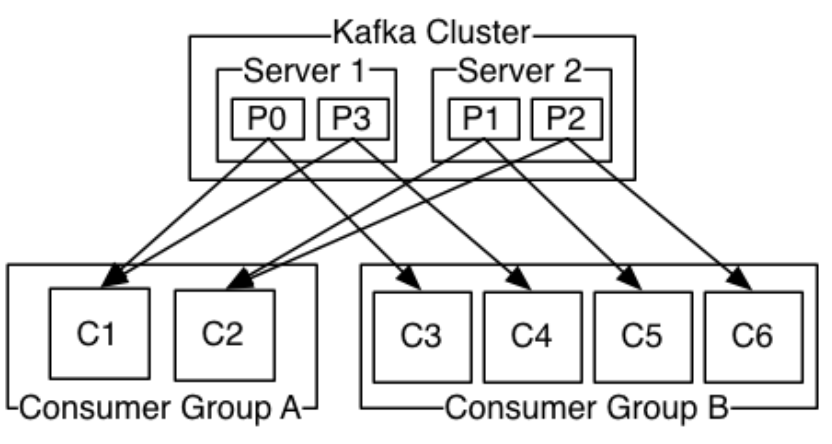
\includegraphics[width=80mm]{../kafkaConsumers.png}
    \caption{Wisselwerking tussen partities en consumer-groepen, \autocite{Sookocheff2015}}
    
\end{figure}

\autocite{Sookocheff2015} en \autocite{Johansson2016}

\section{RabbitMq}

Een alternatief voor \emph{Kafka} is \emph{RabbitMq}. Dit is software waar men berichten kan plaatsen en ophalen op één of meerdere 'queues'. Ook hier heb je verschillende mogelijkheden van wat het formaat is van de berichten. Het kan zowel een gewone tekst zijn, als een Json-file. 

Wanneer een bericht van een queue wordt gelezen, dan wordt deze verwijderd van de queue. Het is dus niet mogelijk om later opnieuw hetzelfde bericht op te gaan vragen. De volledige queue kan ook een broker genoemd worden. Er zijn hier ook producers die data op de queue zetten, alsook consumers die een subscriptie kunnen maken op een queue. 

\emph{RabbitMq} kan een voordeel zijn om te gebruiken in verschillende situaties. Als je bijvoorbeeld als gebruiker de data die je opslaat in een queue wilt distribueren naar verschillende consumers, dan is ook \emph{RabbitMq} een ideale technologie om dit te doen. Het is dus mogelijk de berichten te versturen naar verschillende consumers. Een ander voordeel is dat het mogelijk is om je berichten te verdelen over verschillende consumers. Op deze manier wordt dan de hoeveelheid mooi gebalanceerd verdeeld over de verschillende consumers.

Er werd hier reeds vermeld dat een queue ook een broker genoemd kan worden. Maar eigenlijk is een broker bij \emph{RabbitMq} iets meer dan dat. Bij een broker kan je ook de exchange mee rekenen. Deze is verantwoordelijk voor het verzenden van de berichten naar de verschillende queues. Indien een bericht in de broker toekomt, moet deze dus eerst langs de exchange voordat hij in een queue terecht kan. De link tussen de queue en de exchange wordt ook wel eens een binding genoemd.

Er zijn vier verschillende soorten van exchanges. Dit zijn: direct, fanout, topic en headers exchanges. Drie van deze worden uitgebeeld in figuur 2.5 \begin{itemize}
    \item De direct exchanges sturen berichten naar een queue op basis van een routing key. Deze key is hetzelfde als de binding key van de queue waarnaar het naartoe moet verzenden. 
    \item Fanout exchanges sturen berichten naar alle queues die verbonden zijn met de exchange
    \item Bij Topic exchanges worden wildcard matches gebruikt . De match wordt gedaan tussen de routing key en de routing pattern die in de binding gespecificeerd wordt.
    \item Header exchanges gebruiken de attributen uit de header om te bepalen welke queue de bestemming is van een bericht.
\end{itemize}
 \begin{figure}[h!]
    \centering
    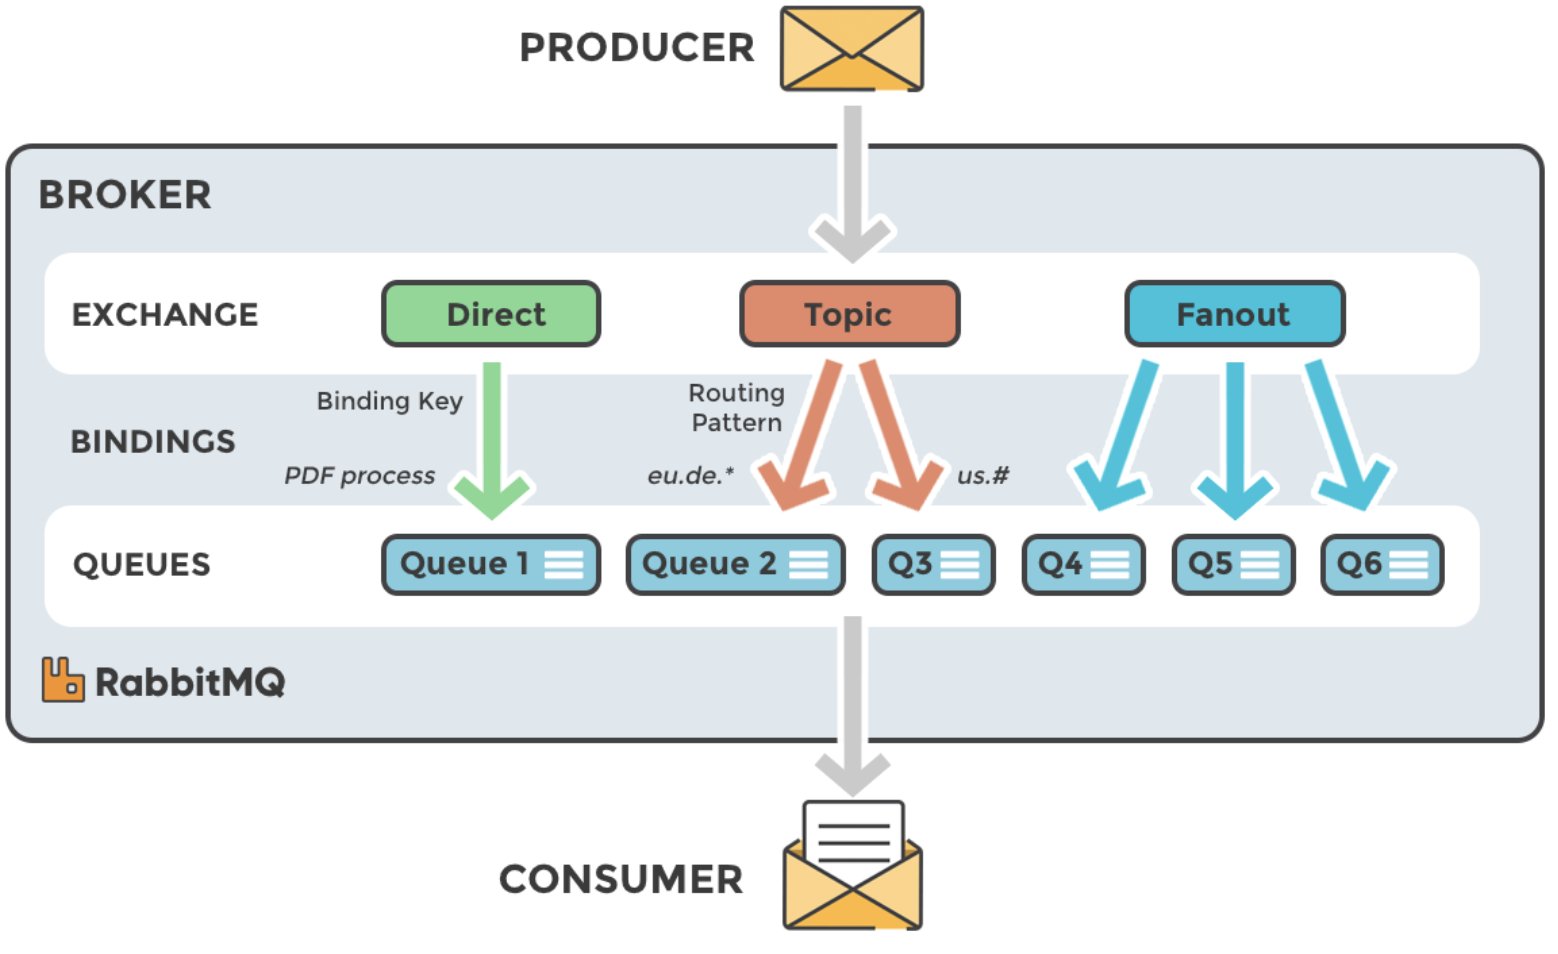
\includegraphics[width=60mm]{../rabbitmqExchanges.png}
    \caption{Werking drie verschillende exchanges bij \emph{RabbitMq}, \autocite{Johansson2015}}
    
\end{figure}
\autocite{Johansson2015}
\section{Kafka vs RabbitMq}
Als we kijken naar Google Trends om te bepalen welke van deze twee technologiën nu het populairste is, dan krijgen we in figuur 2.6 een grafiek te zien van het afgelopen jaar.
 \begin{figure}[h!]
    \centering
    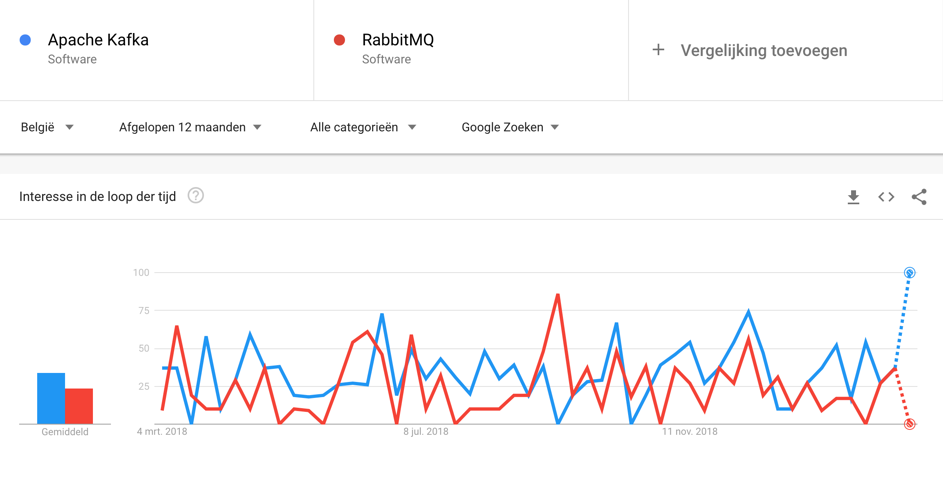
\includegraphics[width=100mm]{../KvsRMQ1.png}
    \caption{Populariteit \emph{Kafka} en \emph{RabbitMq} in het afgelopen jaar, \autocite{Trends2019}}
    
\end{figure}

In deze grafiek is duidelijk te zien dat \emph{Kafka} iets populairder is dan \emph{RabbitMq}. Er zit tussen juli en november wel een piek in waarbij \emph{RabbitMq} veel populairder is, maar over het algemeen gezien kunnen we concluderen dat in het afgelopen jaar \emph{Kafka} toch iet wat populairder is.

 \begin{figure}[h!]
    \centering
    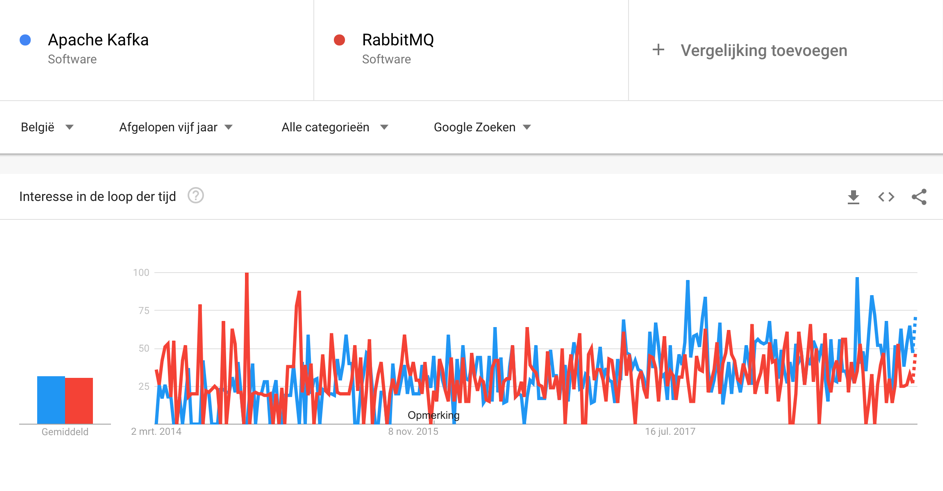
\includegraphics[width=100mm]{../KvsRMQ2.png}
    \caption{Populariteit \emph{Kafka} en \emph{RabbitMq} in de afgelopen vijf jaar, \autocite{Trends2019}}
    
\end{figure}

Als je figuur 2.7 bekijkt, dan zie je een algemene trend. Namelijk dat vijf jaar geleden \emph{RabbitMq} veel populairder was, maar dat deze trend systematisch omgedraaid is. Uit deze figuur valt ook af te leiden dat in het algemeen de interesse naar technologieën voor microservices lichtjes toegenomen is in de laatste vijf jaar.

\autocite{Trends2019}

\section{Google Pub/Sub}
Tijdens het academiejaar dat dit onderzoek is uitgevoerd, zijn de gebruikte technologieën die TVH gebruikt ook wat veranderd. Er is momenteel een nieuwe technologie bij gekomen, namelijk \emph{Google Pub/Sub}. Zoals de naam doet vermoeden is Google eigenaar van deze technologie. 

Ook hier zijn het ongeveer dezelfde kernwoorden die belangrijk zijn:
\begin{itemize}
    \item Topic
    \item Subscription
    \item Message
    \item Publisher
    \item Subscriber
\end{itemize}

De termen topic en message zijn hetzelfde als bij de andere technologieën. Subscription is de link tussen de subscriber (deze wordt straks uitgelegd), en de topic. Dit is dus een soort van abonnement die een subscriber aangaat met een topic. Een subscriber is iemand of iets die de verschillende messages van een specifieke topic leest. Een publisher is dan degene die nieuwe messages op een topic plaatst.

 \begin{figure}[h!]
    \centering
    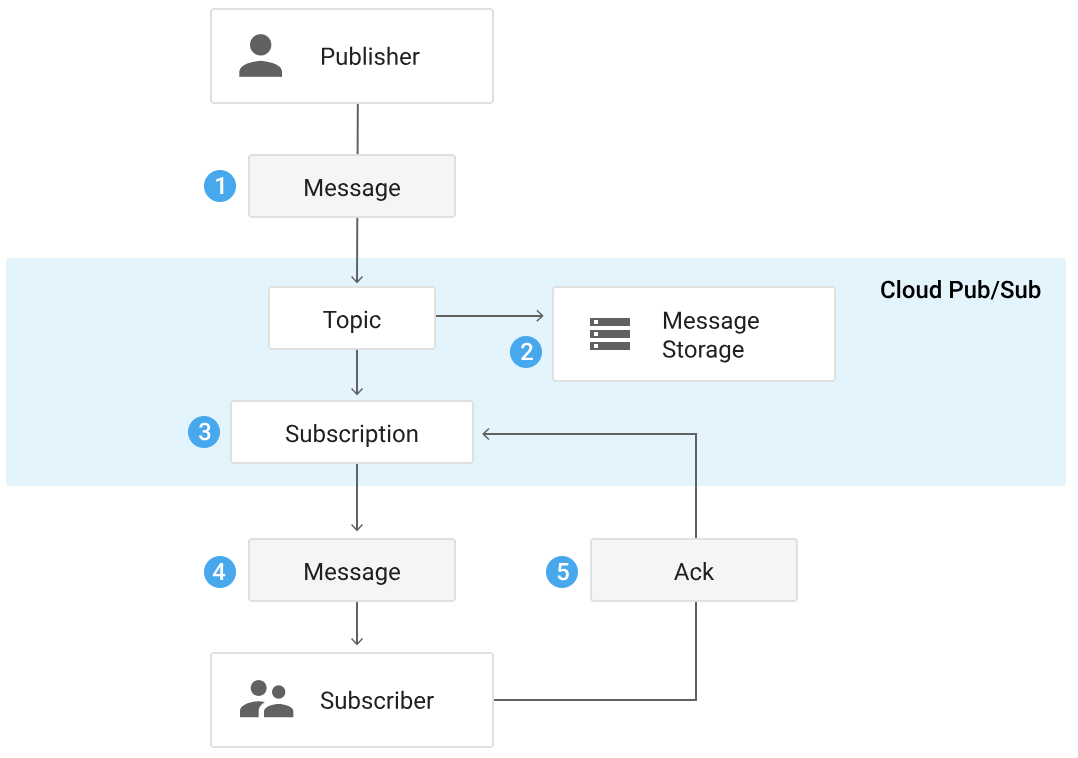
\includegraphics[width=100mm]{../gpsFlow.png}
    \caption{De flow die een message aflegt bij \emph{Google Pub/Sub}, \autocite{Google2019}}
    
\end{figure}

Op figuur 2.8 is te zien hoe een message tot bij een subscriber geraakt, iemand of iets die de message leest. Eerste stap is de publisher die een message plaatst (published) naar een topic. Een message bevat een payload, dit is de inhoud van de message. Ook kan er eventueel attributen toegevoegd worden die iets meer vertellen over de inhoud van de payload. Vervolgens wordt in de tweede stap de message opgeslagen in de Message Storage totdat een subscriber de message leest en acknowledged. Dit wil zeggen dat de subscriber een bevestiging stuurt naar de subscription om te melden dat hij de message goed ontvangen heeft. Hierna zet de Pub/Sub deze message klaar in al zijn subscriptions. Deze message wordt dan gelezen als bijvoorbeeld de subscriber deze message binnen trekt. In de vierde stap zien we dat alle berichten die nog niet gelezen zijn door de subscriber, bij de subscriber binnen komen. Als een message goed is aangekomen, dan wordt er een acknowledge gestuurd naar de subscription. Dan wordt deze message ook verwijderd en kan deze niet meer opnieuw gelezen worden. Dit is de vijfde stap.

\autocite{Google2019}

\section{IoT-applicatie}

\section{TVH}




